

\section{The OS Library Components}\label{section:oslibrary}\index{OSLibrary@{\tt OSLibrary}|(} 

\subsection{OSAgent}\label{section:osagent}

The {\tt OSAgent}\index{OSAgent@{\tt OSAgent}|(}  part of the library is used to facilitate communication
with remote solvers. It is not used if the solver is invoked locally (i.e., on the same machine).
There are two key classes in the {\tt OSAgent} component of the OS library. The two classes are
{\tt OSSolverAgent}\index{OSSolverAgent@{\tt OSSolverAgent}} and {\tt WSUtil}\index{WSUtil@{\tt WSUtil}}.

The {\tt OSSolverAgent} class is used to contact a remote solver service.  For example, assume that {\tt sOSiL}
is a string with a problem instance and {\tt sOSoL} is a string with solver options. Then the following code
will call a solver service and invoke the {\tt solve} method.
\begin{verbatim}
OSSolverAgent *osagent;
string serviceLocation = http://kipp.chicagobooth.edu/os/OSSolverService.jws
osagent = new OSSolverAgent(  serviceLocation );
string sOSrL = osagent->solve(sOSiL, sOSoL);
\end{verbatim}
Other methods in the {\tt OSSolverAgent} class are {\tt send}, {\tt retrieve}, {\tt getJobID}, {\tt knock}, and {\tt kill}.  
The use of these methods is described in Section~\ref{section:servicemethods}.



The methods in the {\tt OSSolverAgent} class call methods in the {\tt WSUtil} class that perform such tasks as 
creating and parsing SOAP messages and making low level socket calls to the server running the solver service. 
The average user will not use methods in the {\tt WSUtil} class, but they are available to anyone wanting to make socket calls or create SOAP messages.

There is also a method, {\tt OSFileUpload}, in the OSAgentClass that is used to upload files from the hard drive of a client to the server. 
It is very fast and does not involve SOAP or Web Services. The {\tt OSFileUpload}  method is illustrated and described in the example code 
{\tt OSFileUpload.cpp} described in Section~\ref{section:fileupload}.
\index{OSAgent@{\tt OSAgent}|)}

\subsection{OSCommonInterfaces}

The classes in the OSCommonInterfaces component of the OS library are used to read and write files and strings
in the OSiL and OSrL protocols. See Section~\ref{section:schemadescriptions} for more detail on OSiL, OSrL,
and other OS protocols. For a complete listing of all of the files in {\tt OSCommonInterfaces} see the 
Doxygen\index{Doxygen} documentation we deposited at {\tt\UrlDoxygen}. Users who have Doxygen installed on their system
can also create their own version of the documentation (see Section~\ref{section:documentation}). Below we highlight 
some key classes.





\subsubsection{The OSInstance Class}\label{section:osinstanceclass}

The OSInstance\index{OSInstance@{\tt OSInstance}|(} class is the in-memory representation of an optimization instance and is a key
class for users of the OS project. This class has an API defined by a collection of {\tt get()} methods for
extracting various components (such as bounds and coefficients) from a problem instance, a collection of
{\tt set()} methods for modifying or generating an optimization instance, and a collection of {\tt calculate()}
methods for function, gradient, and Hessian evaluations.  See Section~\ref{section:osinstanceAPI}.
We now describe how to create an {\tt OSInstance} object and the close relationship between the OSiL\index{OSiL} schema
and the {\tt OSInstance} class.

\subsubsection{Creating an {\tt OSInstance} Object}

The OSCommonInterfaces component contains an {\tt OSiLReader}  class for reading an instance in an OSiL string and
creating an in-memory {\tt OSInstance} object.  Assume that {\tt sOSiL} is a string that will hold the instance in OSiL format. Creating an {\tt OSInstance} object is illustrated in Figure~\ref{figure:creatingosinstanceobject}.

\begin{figure}[ht]
\centering
   \small {\obeyspaces\let =\
\fbox{\tt\begin{tabular}{@{}l@{}}
OSiLReader *osilreader = NULL;\\[\Sb]
OSInstance *osinstance = NULL;\\[\Sb]
osilreader = new OSiLReader();\\[\Sb]
osinstance = osilreader->readOSiL( sOSiL);\\[\Sb]
\end{tabular} }} \bigskip
\caption{Creating an {\tt OSInstance} Object} \label{figure:creatingosinstanceobject}
\end{figure}

\subsubsection{Mapping Rules}\label{section:mappingrules}

The {\tt OSInstance} class has two members, {\tt instanceHeader} and {\tt instanceData}.  
These correspond to the XML elements {\tt <instanceHeader>} and {\tt <instanceData>}.
They are of type {\tt InstanceHeader} and {\tt InstanceData}, respectively, which in turn  
correspond to the OSiL schema's complexTypes {\tt InstanceHeader} and {\tt InstanceData}, and 
in themselves are C++ classes.

    Moving down one level, Figure~\ref{figure:instancedata} shows that the {\tt InstanceData} class has in turn 
the members {\tt variables}, {\tt objectives}, {\tt constraints}, {\tt linearConstraintCoefficients}, 
{\tt quadraticCoefficients}, and {\tt nonlinearExpressions}, corresponding to the respective elements 
in the OSiL file that have the same name. Each of these are instances of associated classes which correspond
to complexTypes in the OSiL schema.


\begin{figure}[ht]
\centering
   \small {\obeyspaces\let =\
\fbox{\tt\begin{tabular}{@{}l@{}}
class OSInstance\{\\[\Sb]
public:\\[\Sb]
     OSInstance(); \\[\Sb]
     InstanceHeader *instanceHeader;\\[\Sb]
     InstanceData *instanceData;    \\[\Sb]
\}; //class OSInstance\\[\Sb]
\end{tabular} }} \bigskip
\caption{The {\tt OSInstance} class} \label{figure:osinstance}
\end{figure}


\begin{figure}[ht]
\centering
   \small {\obeyspaces\let =\
\fbox{\tt\begin{tabular}{@{}l@{}}
class InstanceData\{\\[\Sb]
public:\\[\Sb]
     InstanceData();\\[\Sb]
     Variables *variables;\\[\Sb]
     Objectives *objectives;\\[\Sb]
     Constraints *constraints;\\[\Sb]
     LinearConstraintCoefficients *linearConstraintCoefficients;\\[\Sb]
     QuadraticCoefficients *quadraticCoefficients;\\[\Sb]
     NonlinearExpressions *nonlinearExpressions;\\[\Sb]
\}; // class InstanceData
\end{tabular} }} \bigskip
\caption{The {\tt InstanceData} class} \label{figure:instancedata}
\end{figure}


\begin{figure}[hb]
%\includegraphics[scale=0.8]{../../figures/paradigm1.eps}
\centering
   \scriptsize {\obeyspaces\let =\
\fbox{\tt\begin{tabular}{@{}l@{}}
\textsf{\textbf{Schema complexType  \hspace{3.64in}  In-memory class}}\\[\Sa]
<xs:complexType name="Variables">  <-------------------------------------------->  class Variables\{\\[\Sb]
                                                                                   public:\\[\Sb]
  <xs:sequence>                                                                      Variables();\\[\Sb]
    <xs:element name="var" type="Variable" maxOccurs="unbounded"/>  <----------->    Variable *var;\\[\Sb]
  </xs:sequence>                                                                   \\[\Sb]
  <xs:attribute name="numberOfVariables" type="xs:nonnegativeInteger"                 \\[\Sb]
                use="required"/>  <--------------------------------------------->    int numberOfVariables;\\[\Sb]
</xs:complexType>                                                                  \}; // class Variables\\[\Sb]
 \\[\Sb]
 \\[\Sb]
<xs:complexType name="Variable">  <--------------------------------------------->  class Variable\{\\[\Sb]
                                                                                   public:\\[\Sb]
                                                                                     Variable();\\[\Sb]
  <xs:attribute name="name" type="xs:string" use="optional"/>  <---------------->    string name;\\[\Sb]
  <xs:attribute name="type" use="optional" default="C">  <---------------------->    char type;\\[\Sb]
    <xs:simpleType>\\[\Sb]
      <xs:restriction base="xs:string">\\[\Sb]
        <xs:enumeration value="C"/>\\[\Sb]
        <xs:enumeration value="B"/>\\[\Sb]
        <xs:enumeration value="I"/>\\[\Sb]
        <xs:enumeration value="S"/>\\[\Sb]
        <xs:enumeration value="D"/>\\[\Sb]
        <xs:enumeration value="J"/>\\[\Sb]
      </xs:restriction>\\[\Sb]
    </xs:simpleType>\\[\Sb]
  </xs:attribute>\\[\Sb]
  <xs:attribute name="lb" type="xs:double" use="optional" default="0"/>  <------>    double lb;\\[\Sb]
  <xs:attribute name="ub" type="xs:double" use="optional" default="INF"/>  <---->    double ub;\\[\Sb]
</xs:complexType>                                                                  \}; // class Variable\\[\Sb]
 \\[\Sb]
 \\[\Sb]
\textsf{\textbf{OSiL elements          \hspace{1.83in}  In-memory objects}}\\[\Sa]
<variables numberOfVariables="2">                   OSInstance *osinstance;\\[\Sb]
   <var lb="0" name="x0" type="C"/>                 osinstance->instanceData->variables->numberOfVariables=2;\\[\Sb]
   <var lb="0" name="x1" type="C"/>                 osinstance->instanceData->variables->var=new Variable*[2];\\[\Sb]
</variables>                                        osinstance->instanceData->variables->var[0]->lb=0;\\[\Sb]
                                                    osinstance->instanceData->variables->var[0]->name="x0";\\[\Sb]
                                                    osinstance->instanceData->variables->var[0]->type={\rm 'C'};\\[\Sb]
                                                    osinstance->instanceData->variables->var[1]->lb=0;\\[\Sb]
                                                    osinstance->instanceData->variables->var[1]->name="x1";\\[\Sb]
                                                    osinstance->instanceData->variables->var[1]->type={\rm 'C'};
\end{tabular} }} \medskip\\[\Sb]
\caption{The {\tt <variables>} element as an {\tt OSInstance} object} \label{figure:osinstancevariables}
\end{figure}


Figure~\ref{figure:osinstancevariables} uses the {\tt Variables} class to provide a closer look 
at the correspondence between schema and class. On the right, the {\tt Variables} class contains 
the data member {\tt numberOfVariables} and a pointer to the object {\tt var} of class {\tt Variable}. 
The {\tt Variable} class has  data members {\tt lb} (double), {\tt ub} (double), {\tt name} (string), 
and {\tt type} (char). On the left the corresponding XML {\tt complexType}s are shown, with arrows indicating 
the correspondences. The following rules describe the mapping between the OSiL schema and the 
{\tt OSInstance} class. 
(In order to facilitate the mapping, we insist in the schema construction that every {\tt complexType} be named, 
even though this is not strictly necessary in XML.)
%
\begin{itemize}

\item  Each {\tt complexType} in an OSiL schema corresponds to a class in {\tt OSInstance}.
Thus the OSiL schema's {\tt complexType} {\tt Variables} corresponds to {\tt OSInstance}'s class {\tt Variables}.
Elements in an actual XML file then correspond to objects in {\tt OSInstance};
for example, the {\tt <variables>} element that is of type {\tt Variables} in an OSiL file
corresponds to a {\tt variables} object in {\tt OSInstance}. 
%(Since {\tt <variables>} is an element of the
%element {\tt <instanceData>} in OSiL, the {\tt variables} object is contained in class {\tt instanceData}.)

\item An attribute or element used in the definition of a {\tt complexType} is a member of the 
corresponding {\tt OSInstance} class, and the type of the attribute or element matches the type 
of the member.  In Figure~\ref{figure:osinstancevariables}, for example, {\tt lb} is an attribute 
of the OSiL {\tt complexType} named {\tt Variable}, and {\tt lb} is a member of the {\tt OSInstance} 
class {\tt Variable}; both have type {\tt double}.  Similarly, {\tt <var>} is an element in the definition 
of the OSiL {\tt complexType} named {\tt Variables}, and {\tt var} is a member of the {\tt OSInstance} 
class {\tt Variables}; the {\tt <var>} element has type {\tt Variable} and the {\tt var} member is a 
{\tt Variable} object.

\item A schema sequence corresponds to an array. For example, in Figure~\ref{figure:osinstancevariables} the complexType {\tt Variables} has a sequence of {\tt <var>} elements that are of type {\tt Variable}, and the corresponding {\tt Variables} class has a member that is an array of type {\tt Variable}.

\item
XML allows a wide range of data subtypes, which do not always have counterparts in the {\tt OSInstance} object.
For instance, the attribute {\tt type} in the {\tt <var>} element forms an enumeration, while the corresponding
member of the {\tt Variable} class is declared as {\tt char}. 

\item
XML allows default values for optional attributes; these default values can be set inside of the constructor of the corresponding data member. 
\end{itemize}
%
General nonlinear terms are stored in the data structure as {\tt OSExpressionTree} objects, which are the subject of the next section.

     The {\tt OSInstance} class has a collection of {\tt get()}, {\tt set()}, and {\tt calculate()} methods 
that act as an API for the optimization instance and are described in Section~\ref{section:osinstanceAPI}.




\subsubsection{The OSExpressionTree OSnLNode Classes}\label{section:osexpressiontreeclass}

The {\tt OSExpressionTree}\index{OSExpressionTree@{\tt OSExpressionTree}} class provides the in-memory representation
of the nonlinear terms.  Our design goal is  to allow for efficient parsing of OSiL\index{OSiL} instances,
while providing an API that meets the needs of diverse solvers.  Conceptually, any nonlinear expression in the
objective or constraints is represented by a tree.  The expression tree for the nonlinear part of the
objective function~(\ref{eq:roobj}), for example, has the form illustrated in Figure~\ref{figure:expressiontree}.
The choice of a data structure to store such a tree --- along with the associated methods of an API --- is a key aspect
in the design of the {\tt OSInstance} class.

\begin{figure}[ht]
\centering
%\includegraphics[scale=0.38]{\figurepath/expressiontree.png}
\includegraphics[scale=0.38]{./figures/expressiontree.png}
\caption{Conceptual expression tree for the nonlinear part of the objective (\ref{eq:roobj}).}\label{figure:expressiontree}
\end{figure}


A base abstract class {\tt OSnLNode} is defined and  all of an OSiL file's
operator and operand elements used in defining a
nonlinear expression are extensions of the base element type {\tt OSnLNode}. There is an element type {\tt OSnLNodePlus}, 
for example, that extends {\tt OSnLNode}; then in an OSiL instance file, there are {\tt <plus>} elements that 
are of type {\tt OSnLNodePlus}.   Each {\tt OSExpressionTree} object contains a pointer to an {\tt OSnLNode} object 
that is the root of the corresponding expression tree.  To every element that extends the {\tt OSnLNode} type in an 
OSiL instance file, there corresponds a class that derives from the {\tt OSnLNode} class in an {\tt OSInstance} 
data structure.  Thus we can construct an expression tree of homogenous nodes, and methods that operate on the 
expression tree to calculate function values, derivatives, postfix notation, and the like do not require switches 
or complicated logic.


\begin{figure}[ht]
\centering
   \small {\obeyspaces\let =\
\fbox{\tt\begin{tabular}{@{}l@{}}
   double OSnLNodePlus::calculateFunction(double *x)\{\\[\Sb]
      m\_dFunctionValue = \\[\Sb]
         m\_mChildren[0]->calculateFunction(x) +\\[\Sb]
         m\_mChildren[1]->calculateFunction(x);\\[\Sb]
      return m\_dFunctionValue;\\[\Sb]
   \} //calculateFunction\\[\Sb]
\end{tabular} }} \medskip
\caption{The function calculation method for the {\tt plus} node class with polymorphism}
   \vspace{-8pt} \label{figure:calcfunction}
\end{figure}


The {\tt OSInstance} class has a variety of {\tt calculate()} methods, based on two pure virtual functions 
in the {\tt OSInstance} class.  The first of these, {\tt calculateFunction()}, takes an array of {\tt double} 
values corresponding to decision variables, and evaluates the expression tree for those values.  Every class
that extends {\tt OSnLNode} must implement this method.  As an example, the {\tt calculateFunction} method 
for the {\tt OSnLNodePlus} class is shown in Figure~\ref{figure:calcfunction}.  Because the OSiL instance 
file must be validated against its schema, and in the schema each {\tt <OSnLNodePlus>} element is specified 
to have exactly two child elements, this {\tt calculateFunction} method can assume that there are exactly 
two children of the node that it is operating on.  The use of polymorphism and recursion makes adding new 
operator elements easy; it is simply a matter of adding a new class and implementing the {\tt calculateFunction()} 
method for it.



Although in the OSnL schema, there are 200+ nonlinear operators, only the following {\tt  OSnLNode} classes are currently supported in our implementation.

\begin{itemize}
\item OSnLNodeVariable
\item OSnLNodeTimes
\item OSnLNodePlus
\item OSnLNodeSum
\item OSnLNodeMinus
\item OSnLNodeNegate
\item OSnLNodeDivide
\item OSnLNodePower
\item OSnLNodeProduct
\item OSnLNodeLn
\item OSnLNodeSqrt
\item OSnLNodeSquare
\item OSnLNodeSin
\item OSnLNodeCos
\item OSnLNodeExp
\item OSnLNodeIf
\item OSnLNodeAbs
\item OSnLNodeMax
\item OSnLNodeMin
\item OSnLNodeE
\item OSnLNodePI
\item OSnLNodeAllDiff
\end{itemize}
\index{OSInstance@{\tt OSInstance}|)}



\subsubsection{The OSOption Class}\label{section:osoptionclass}

The {\tt OSOption}\index{OSOption@{\tt OSOption}|(} class is the in-memory representation of the options 
associated with a particular optimization task. It is another key
class for users of the OS project. This class has an API defined by a collection of {\tt get()} methods for
extracting various components (such as initial values for decision variables, solver options, job parameters, etc.), 
and a collection of {\tt set()} methods for modifying or generating an option instance. The relationship between
in-memory classes and objects on one hand and complexTypes and elements of the OSoL schema follow the same mapping rules
laid out in Section~\ref{section:mappingrules}.
\index{OSOption@{\tt OSOption}|)}

\subsubsection{The OSResult Class}\label{section:osresultclass}

Similarly the {\tt OSResult}\index{OSResult@{\tt OSResult}|(} class is the in-memory representation of the 
results returned by the solver and other information associated with a particular optimization task. 
This class has an API defined by a collection of {\tt set()} methods that allow a solver to create a result instance
and a collection of {\tt get()} methods for
extracting various components (such as optimal values for decision variables, optimal objective function value, 
optimal dual variables, etc.). The relationship between
in-memory classes and objects on one hand and complexTypes and elements of the OSoL schema follow the same 
mapping rules laid out in Section~\ref{section:mappingrules}.
\index{OSResult@{\tt OSResult}|)}



\subsection{OSModelInterfaces}\label{section:osmodelinterfaces}

This part of the OS library is designed to help integrate the OS standards with other standards and modeling systems.

\subsubsection{Converting MPS Files}

The MPS standard\index{MPS format|(} is still a popular format for representing linear and integer programming problems.
In {\tt OSModelInterfaces,} there is a class {\tt OSmps2osil}\index{OSmps2osil@{\tt OSmps2osil}|(} that can be used
to convert files in MPS format into the OSiL\index{OSiL} standard. It is used as follows.

\begin{verbatim}
OSmps2osil *mps2osil = NULL;
DefaultSolver *solver  = NULL;
solver = new CoinSolver();
solver->sSolverName = "cbc";
mps2osil = new OSmps2osil(  mpsFileName);
mps2osil->createOSInstance() ;
solver->osinstance = mps2osil->osinstance;
solver->solve();
\end{verbatim}

The {\tt OSmps2osil} class constructor takes a string which should be the
file name of the instance in MPS format. The constructor then uses the
{\tt CoinUtils}\index{COIN-OR projects!CoinUtils@{\tt CoinUtils}} library to read and parse the MPS file.  The class method {\tt createOSInstance} then builds  an in-memory {\tt osinstance} object  that can be used by a solver.
\index{OSmps2osil@{\tt OSmps2osil}|)}\index{MPS format|)}

\subsubsection{Converting AMPL nl Files}\label{section:nl2osil}

AMPL is a popular modeling language that saves  model instances in the AMPL nl format\index{AMPL nl format|(}.
The {\tt OSModelInterfaces} library provides a class, {\tt OSnl2osil}\index{OSnl2osil@{\tt OSnl2osil}},
for reading an nl file and creating a
corresponding in-memory  {\tt osinstance}\index{OSInstance@{\tt OSInstance}} object. It is used as follows.

\begin{verbatim}
OSnl2osil *nl2osil = NULL;
DefaultSolver *solver  = NULL;
solver = new LindoSolver();
nl2osil = new OSnl2osil( nlFileName);
nl2osil->createOSInstance() ;
solver->osinstance = nl2osil->osinstance;
solver->solve();
\end{verbatim}


The {\tt OSnl2osil} class works much like the {\tt OSmps2osil}\index{OSmps2osil@{\tt OSmps2osil}} class. The
{\tt OSnl2osil} class constructor takes a string which should be the file name of the instance in nl format. The constructor then uses the AMPL ASL library routines to read and parse the nl file. The class method {\tt createOSInstance} then builds  an in-memory {\tt osinstance} object  that can be used by a solver.

In Section~\ref{section:amplclient}  we describe the {\tt OSAmplClient}\index{OSAmplClient@{\tt OSAmplClient}}
executable that acts as a ``solver'' for AMPL. The {\tt OSAmplClient} uses the {\tt OSnl2osil} class to convert
the instance in nl format to OSiL\index{OSiL} format before calling a solver either locally or remotely.
\index{AMPL nl format|)}


\subsection{OSParsers}\label{section:osparsers}

The OSParsers component of the OS library contains reentrant parsers that  read OSiL\index{OSiL|(},
OSoL\index{OSoL} and OSrL\index{OSrL} strings and build, respectively, in-memory 
OSInstance\index{OSInstance@{\tt OSInstance}}, OSOption\index{OSOption@{\tt OSOption}} and 
OSResult\index{OSResult@{\tt OSResult}}  objects.


The OSiL parser is invoked through an {\tt OSiLReader} object as illustrated below. Assume {\tt osil} is a string with the problem instance.
\begin{verbatim}
OSiLReader *osilreader = NULL;
OSInstance *osinstance = NULL;
osilreader = new OSiLReader();
osinstance = osilreader->readOSiL( osil);
\end{verbatim}
The {\tt  readOSiL} method  has a single argument which is a (pointer to a) string. 
The {\tt  readOSiL} method then calls an underlying method {\tt yygetOSInstance} that parses the OSiL string. 
The major components of the OSiL schema  recognized by the parser are
\begin{verbatim}
<instanceHeader>
<instanceData>
<variables>
<objectives>
<constraints>
<linearConstraintCoefficients>
<quadraticCoefficients>
<nonlinearExpressions>
\end{verbatim}
There are other components in the OSiL\index{OSiL|)} schema, but they are not yet implemented.
In most large-scale applications the {\tt <variables>,} {\tt <objectives>}, {\tt <constraints>}, and {\tt <linearConstraintCoefficients>}
will comprise the bulk of the instance memory.  Because of this, we have ``hard-coded'' the OSiL parser
to read these specific elements very efficiently.
The parsing of the {\tt <quadraticCoefficients>} and {\tt <nonlinearExpressions>} is done using code generated
by {\tt flex}\index{flex@{\tt flex}} and {\tt bison}\index{bison@{\tt bison}}. The file  
{\tt OSParseosil.l} is used by {\tt flex}\index{flex@{\tt flex}} to generate {\tt OSParseosil.cpp} and the file 
{\tt OSParseosil.y} is used by {\tt bison}\index{bison@{\tt bison}} to generate {\tt OSParseosil.tab.cpp}.
In {\tt OSParseosil.l} we use the {\tt reentrant} option and in {\tt OSParseosil.y} we use the
{\tt pure-parser} option to generate reentrant parsers. The {\tt OSParseosil.y} file  contains both our
``hard-coded'' parser and the grammar rules for the  {\tt <quadraticCoefficients>} and
{\tt <nonlinearExpressions>} sections.
We are currently using GNU {\tt bison} version 3.2 and {\tt flex} 2.5.33.

The typical OS user will have no need to edit either {\tt OSParseosil.l} or {\tt OSParseosil.y} 
and therefore will not have to worry about running either {\tt flex} or {\tt bison} to generate the parsers. 
The generated parser code from {\tt flex} and {\tt bison} is distributed with the project and works on all 
of the platforms listed in Table~\ref{table:testedplatforms}.  If the user does edit either {\tt parseosil.l} 
or {\tt parseosil.y} then {\tt parseosil.cpp} and {\tt parseosil.tab.cpp} need to be regenerated with 
{\tt flex} and {\tt bison}. If these programs are present, in the OS directory  execute
%
\index{make run_parsers@{\tt make run\_parsers}}
\begin{verbatim}
make  run_parsers
\end{verbatim}
%
(This requires Unix or a unix-like environment (Cygwin, MinGW, MSYS, etc.) under Windows.)

The files {\tt OSParseosrl.l} and {\tt OSParseosrl.y} are used by {\tt flex} and {\tt bison} to  generate the code 
{\tt OSParseosrl.cpp} and {\tt OSParseosrl.tab.cpp} for parsing strings in OSrL format. The comments made above about the 
OSiL parser apply to the OSrL parser. The OSrL parser, like the OSiL parser, is invoked using an {\tt OSrL} reading object.
This is illustrated below ({\tt osrl} is a string in OSrL format).
\begin{verbatim}
OSrLReader *osrlreader = NULL;
osrlreader = new OSrLReader();
OSResult *osresult = NULL;
osresult = osrlreader->readOSrL( osrl);
\end{verbatim}

The OSoL parser follows the same layout and rules.
The files {\tt OSParseosol.l} and {\tt OSParseosol.y} are used by {\tt flex} and {\tt bison} to  generate the code 
{\tt OSParseosol.cpp} and {\tt OSParseosol.tab.cpp} for parsing strings in OSoL format. The OSoL parser
is invoked using an {\tt OSoL} reading object.
This is illustrated below ({\tt osol} is a string in OSoL format).
\begin{verbatim}
OSoLReader *osolreader = NULL;
osolreader = new OSoLReader();
OSOption *osoption = NULL;
osoption = osolreader->readOSoL( osol);
\end{verbatim}


There is also a lexer {\tt OSParseosss.l} for tokenizing the command line for the OSSolverService executable 
described in Section~\ref{section:ossolverservice}.



\subsection{OSSolverInterfaces}\label{section:ossolverinterfaces}


The {\tt OSSolverInterfaces} library is designed to facilitate linking the OS library with various solver APIs.
We first describe how to take a problem instance in OSiL\index{OSiL} format and connect to a solver 
that has a COIN-OR OSI interface. See the OSI project \url{www.projects.coin-or.org/Osi}.
We then describe hooking to the COIN-OR nonlinear code {\tt Ipopt}\index{COIN-OR projects!Ipopt@{\tt Ipopt}}. 
See \url{www.projects.coin-or.org/Ipopt}.
\ifknitro
Finally we describe hooking to two commercial solvers Knitro\index{Knitro} and LINDO\index{LINDO}.
\else
Finally we describe hooking to the commercial solver LINDO\index{LINDO}.
\fi
The OS library has been tested with the following solvers using the Osi Interface.

\begin{itemize}
\item Bonmin
\item Cbc
\item Clp
\item Couenne
\item Cplex
\item DyLP
\item Glpk
\item Ipopt
\item SYMPHONY
\item Vol
\end{itemize}

In the {\tt OSSolverInterfaces} library there is an abstract class
{\tt DefaultSolver} that has the following key members:

\begin{verbatim}
std::string osil;
std::string osol;
std::string osrl;
OSInstance *osinstance;
OSResult   *osresult;
OSOption   *osoption;
\end{verbatim}
and the pure virtual function
\begin{verbatim}
virtual void solve() = 0 ;
\end{verbatim}
In order to use a solver through the COIN-OR {\tt Osi}\index{COIN-OR projects, {\tt Osi}} 
interface it is
necessary to create an object in the {\tt CoinSolver} class which inherits
from the {\tt DefaultSolver} class and implements the appropriate
{\tt solve()} function.  We illustrate with the {\tt Clp} solver.

\begin{verbatim}
DefaultSolver *solver  = NULL;
solver = new CoinSolver();
solver->m_sSolverName = "clp";
\end{verbatim}

Assume that the data file containing the problem has been read into
the string {\tt osil} and the solver options are in the string {\tt osol}.
Then the {\tt Clp} solver is invoked as follows.

\begin{verbatim}
solver->osil = osil;
solver->osol = osol;
solver->solve();
\end{verbatim}

Finally, get the solution in {\tt OSrL} format as follows

\begin{verbatim}
cout << solver->osrl << endl;
\end{verbatim}

\ifknitro   %--------------------------------------------------------------------------
Even though LINDO and Knitro are commercial solvers and do not have a COIN-OR {\tt Osi} interface, these solvers are
used in exactly the same manner as a COIN-OR solver. For example, to invoke the LINDO solver we do the following.

\begin{verbatim}
solver = new LindoSolver();
\end{verbatim}

Similarly for Knitro and Ipopt. In the case of  Knitro, the {\tt KnitroSolver} class inherits from both
{\tt DefaultSolver} class and the Knitro {\tt NlpProblemDef} class. See {\tt\UrlKnitroMan} for more information 
on the Knitro solver C++ implementation and the {\tt NlpProblemDef} class.  Similarly, for Ipopt 
\else

Some commercial solvers, e.g., LINDO\index{LINDO|(}, do not have a COIN-OR {\tt Osi} interface, 
but it is possible to write wrappers so that they can be used in exactly the same manner 
as a COIN-OR solver. For example, to invoke the
LINDO solver we do the following.

\begin{verbatim}
solver = new LindoSolver();
\end{verbatim}
\index{LINDO|)}

A similar call is used for {\tt Ipopt}\index{COIN-OR projects!Ipopt@{\tt Ipopt}}. In this case, 
\fi         %--------------------------------------------------------------------------
the {\tt IpoptSolver} class inherits from both the {\tt DefaultSolver} class and the Ipopt {\tt TNLP} class. See 

\medskip
\noindent{small\tt\UrlIpoptDoc}
\medskip

\noindent for more information on the Ipopt solver C++ implementation and the {\tt TNLP} class.


In the examples above,  the problem instance was assumed to be read from a file into the string {\tt osil}
and then into the class member {\tt solver->osil.} However, everything can be done entirely in memory.
For example, it is possible to use the {\tt OSInstance}\index{OSInstance@{\tt OSInstance}} class to create
an in-memory problem representation and give this representation directly to a solver class that inherits
from {\tt DefaultSolver}. The class member to use is {\tt osinstance.} This is illustrated in the example
given in Section~\ref{section:exampleOSInstanceGeneration}.


\subsection{OSUtils}

The OSUtils component of the OS library contains utility codes. For example, the {\tt FileUtil} class contains
useful methods for reading files into {\tt string} or {\tt char*} and writing files from {\tt string} and {\tt char*}.
The {\tt OSDataStructures} class holds other classes for things such as sparse vectors, sparse Jacobians, and sparse
Hessians. The {\tt MathUtil} class contains a method for converting between sparse matrices in row and column major form.%
\index{OSLibrary@{\tt OSLibrary}|)}

